\begin{figure}[htbp]
\centering 
  \subfloat[Box plot \acs{SCT}.]{
	  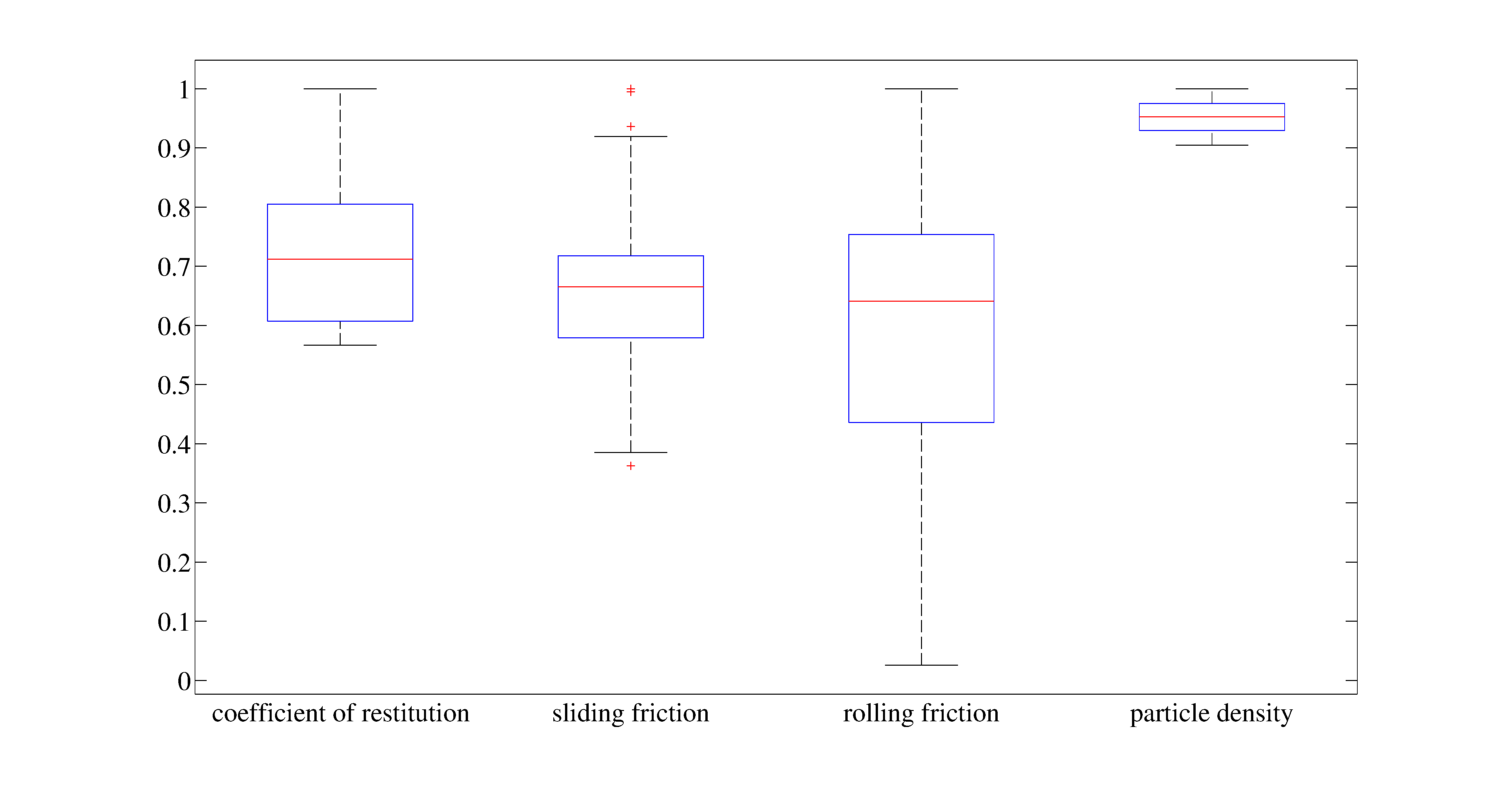
\includegraphics[width=.47\columnwidth]{images/165BoxSCTlimestonefinetest01coeffP1}
	  \label{fig:165BoxSCTlimestonefinetest01coeffP1}
  }
  \quad
  \subfloat[Density plot \acs{SCT}.]{
	  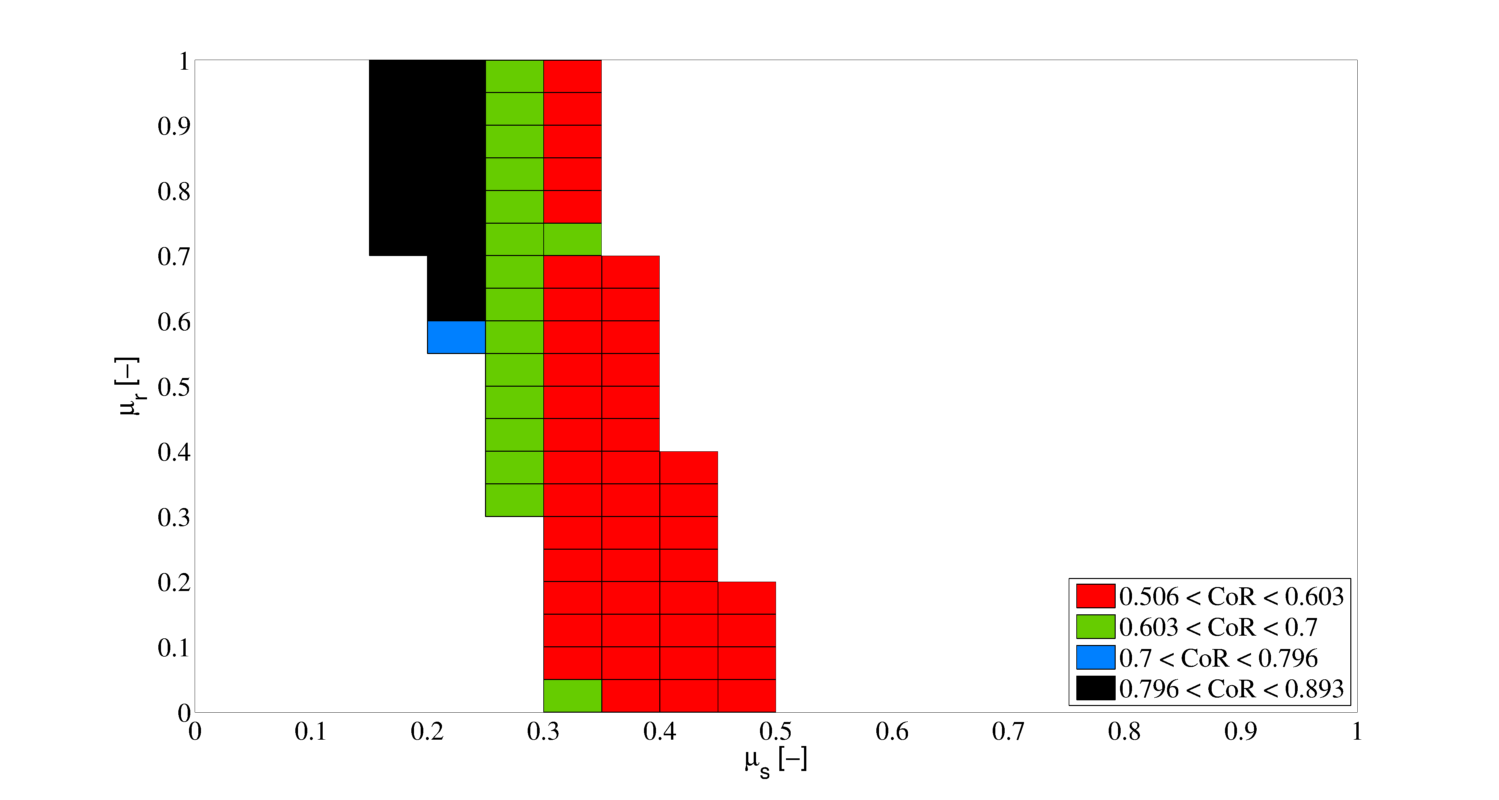
\includegraphics[width=.47\columnwidth]{images/171TileSClimestonefinetest01coef-21}
	  \label{fig:171TileSClimestonefinetest01coef-21}
  }
  \\
    \subfloat[Box plot \acs{AoR}.]{
	  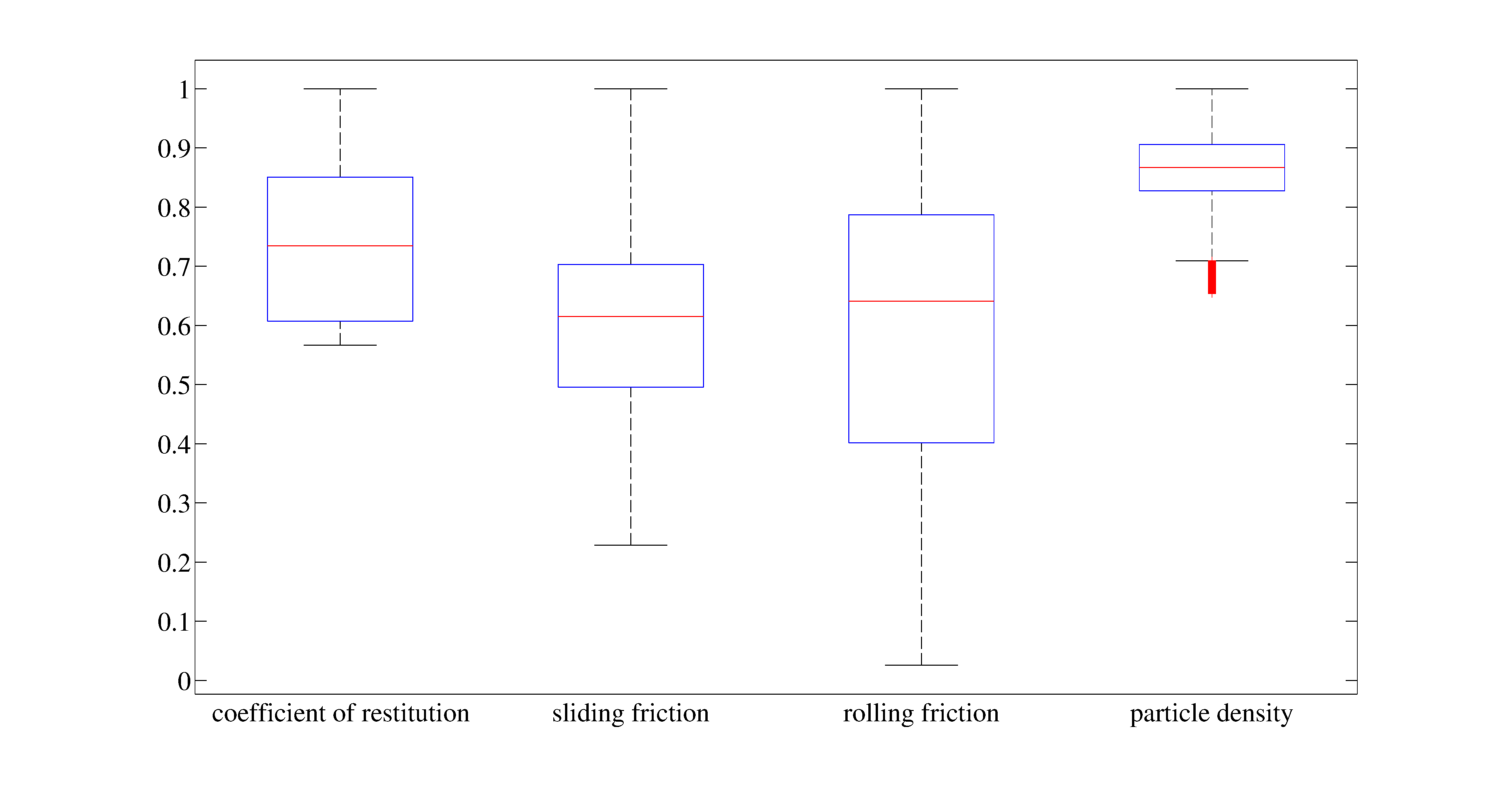
\includegraphics[width=.47\columnwidth]{images/187BoxAORlimestonefine}
	  \label{fig:187BoxAORlimestonefine}  }
  \quad
  \subfloat[Density plot \acs{AoR}.]{
	  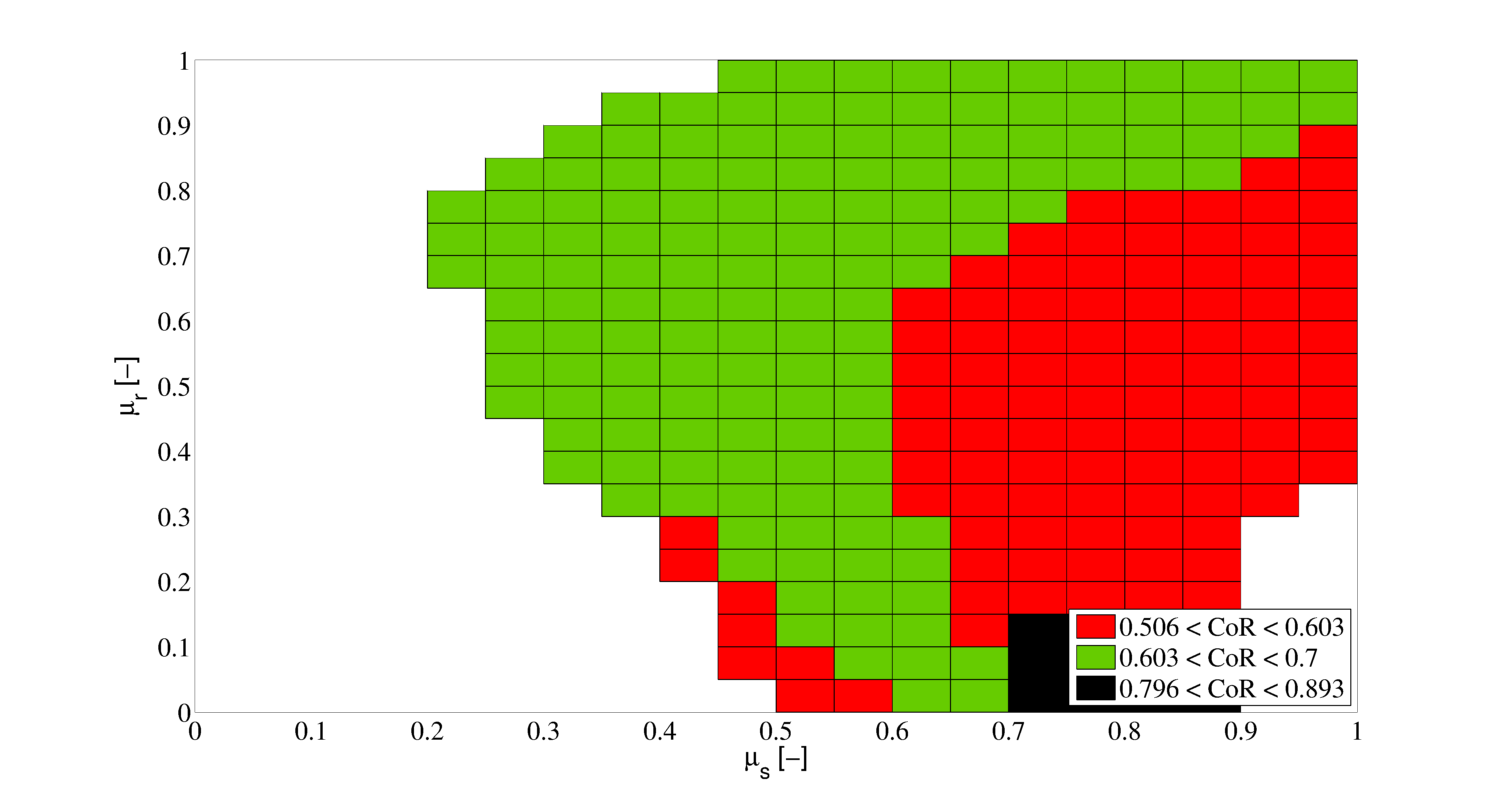
\includegraphics[width=.47\columnwidth]{images/188TileAORlimestonefine}
	  \label{fig:188TileAORlimestonefine}  }
  \\
  \subfloat[Box plot intersection: \acs{AoR} \& \acs{SCT}.]{
	  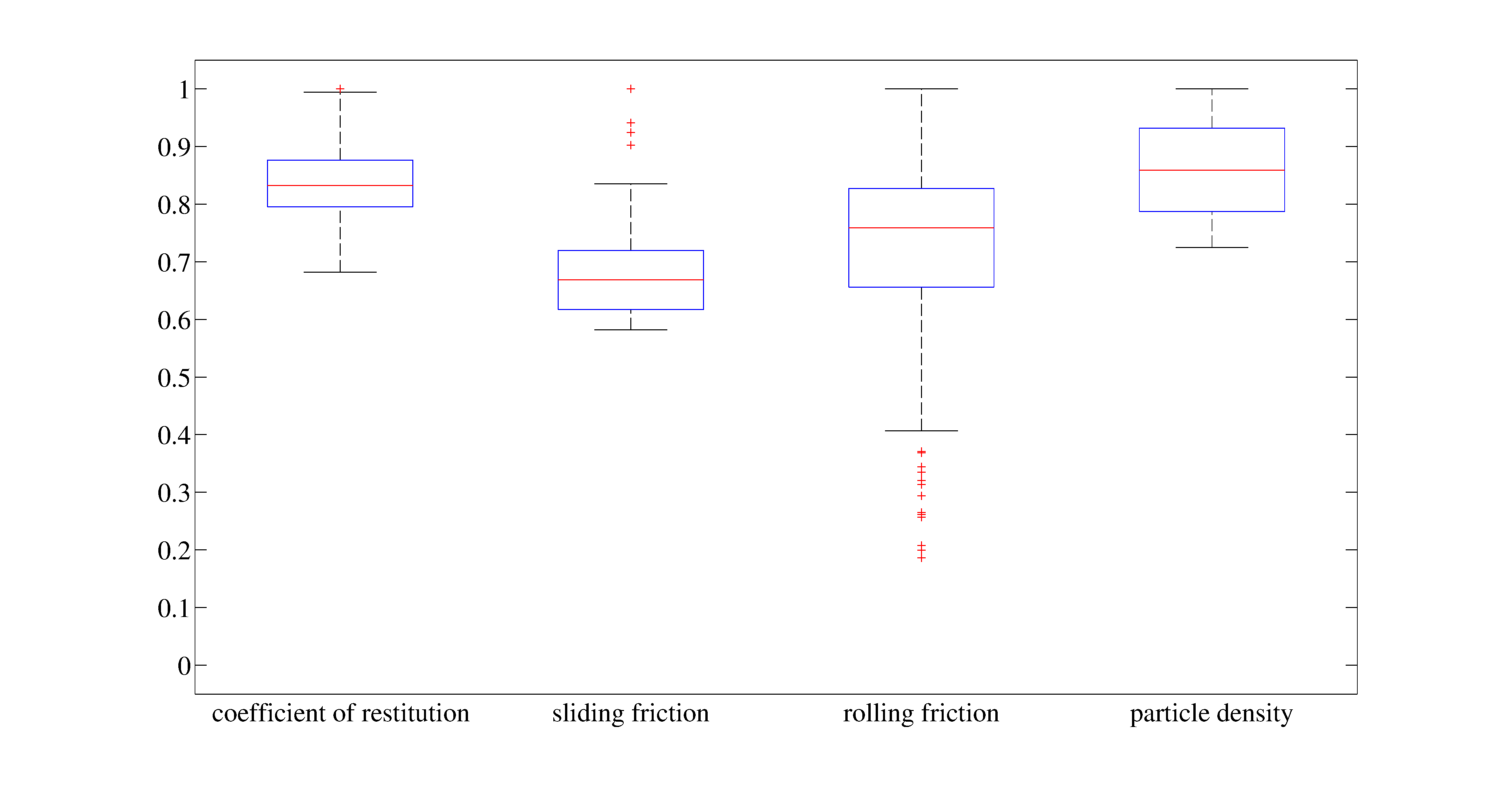
\includegraphics[width=.47\columnwidth]{images/195BoxMixlimestonefine_16}
	  \label{fig:195BoxMixlimestonefine_16}
  }
  \quad
  \subfloat[Density plot intersection: \acs{AoR} \& \acs{SCT}.]{
	  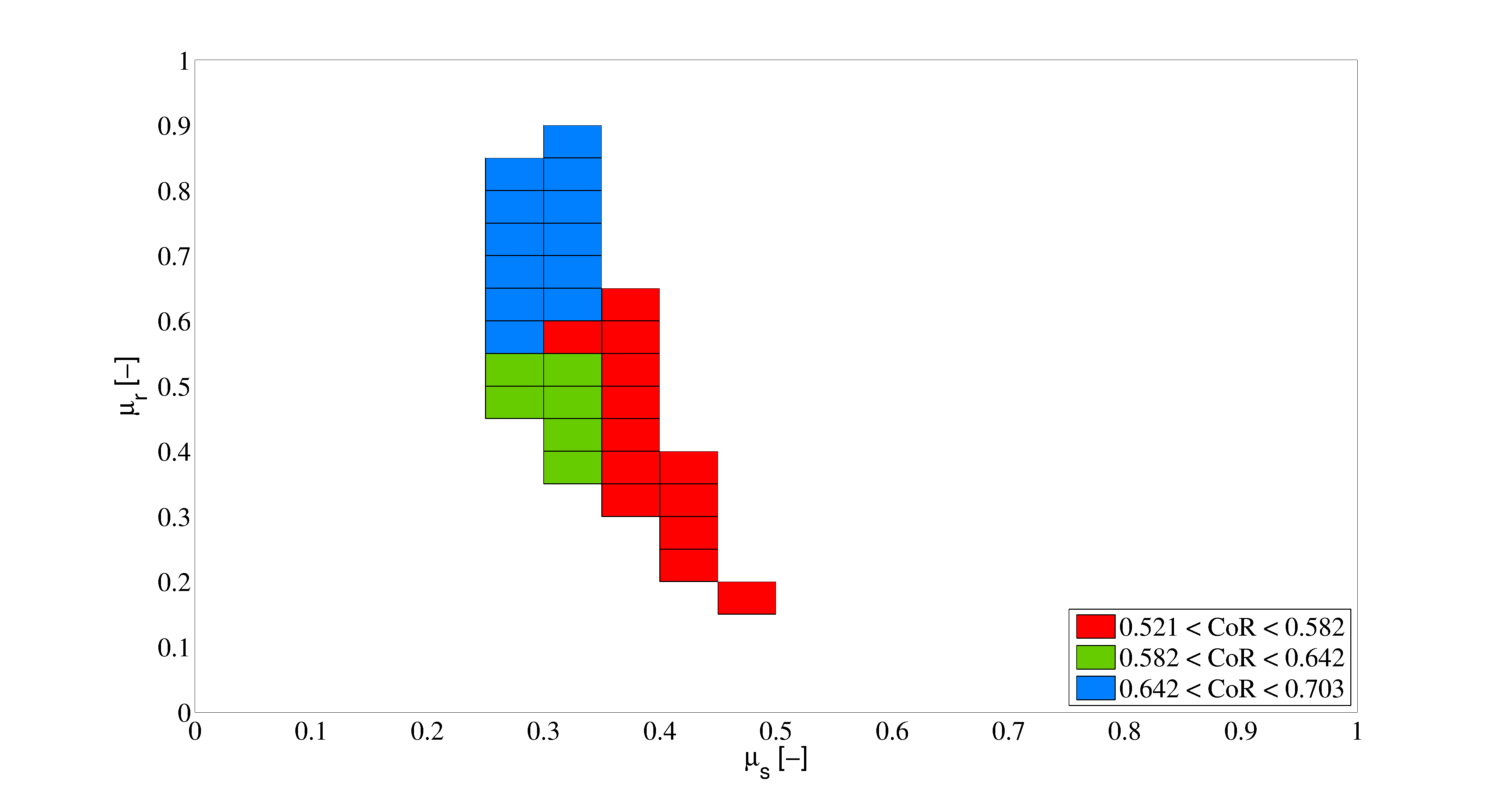
\includegraphics[width=.47\columnwidth]{images/196TileMixlimestonefine_16}
	  \label{fig:196TileMixlimestonefine_16}
  }
  \\    
  \caption[Limestone fine valid values]{Limestone fine valid values. The
  valid values for the \acs{SCT} and \acs{AoR} tests are shown, together with the merge values, valid for both.
  The plots referring to the single test show reasonably narrow confidence
  ranges, while Fig. \ref{fig:195BoxMixlimestonefine_16} shows unreasonably large
  valid ranges. See Section \ref{sec:remainingmaterialscharacterization} for
  the interpretation.}
  \label{fig:219boxplotslimestonefine}
\end{figure}